\chapter{Przecięcie wielokątów}
Problem znalezienia przecięcia dla wielokątów wypukłych zdefiniowany
jest następująco.

\begin{problem}[Przecięcie wielokątów]
  Mając dane dwa wielokąty wypukłe $P$ i $Q$, znaleźć ich
  \emph{przecięcie}, tj.\ obszar należący jednocześnie do $P$ i do
  $Q$.
\end{problem}

W niniejszym rozdziale do wielokąta będziemy zaliczać jego wnętrze
wraz z brzegiem. Jako $n$ będziemy oznaczać liczbę wierzchołków $P$, a
jako $m$ liczbę wierzchołków $Q$. Stosując algorytm naiwny polegający
na sprawdzeniu przecięcia każdej krawędzi $P$ z każdą krawędzią $Q$
można uzyskać punkty wszystkich przecięć w czasie $O(nm)$. Dla
wielokątów prostych ten problem można rozwiązać w czasie
liniowo-logarytmicznym, uprzednio przekształcając go do problemu
przecięcia odcinków, które wymaga czasu liniowego~\cite{Prep85}.

\section{Algorytm Shamosa-Hoeya}
Podstawową metodą rozwiązywania problemów w algorytmice jest technika
\emph{dziel i zwyciężaj}, które polega na podziale na mniejsze części,
znajdowaniu rozwiązań częściowych, a następnie łączeniu ich w końcowy
rezultat.

Metodę wykorzystującą podział płaszczyzny dla problemu przecięcia
wielokątów zaproponowali Shamos i Hoey~\cite{ShamosHoey76}. Przez
każdy wierzchołek $P$ i $Q$ prowadzimy prostą pionową, tworząc w ten
sposób $n+m$ nieskończonych prostokątów zwanych dalej \emph{pasami}
(rysunek~\ref{img:ShamosHoey76}). Znalezienie przecięć krawędzi obydwu
wielokątów w każdej warstwie pozwoli nam na proste wyznaczenie obszaru
przecięcia tych wielokątów. Wynika to z poniższego twierdzenia.

\begin{twierdzenie}[Shamos-Hoey 1976]
  Przecięcie wielokątów wypukłych $P = (p_1, \ldots, p_n)$ i $Q =
  (q_1, \ldots, q_m)$ jest wielokątem wypukłym o sumie wierzchołków
  nie większej niż $n + m$.
\end{twierdzenie}

\begin{proof}
  Przecięcie $P$ i $Q$ jest przecięciem $n + m$ wewnętrznym
  półpłaszczyzn wyznaczonych przez krawędzie obydwu wielokątów.
\end{proof}

Zauważmy, że w każdym pasie proste go ograniczające wraz z krawędziami
wielokąta tworzą trójkąt lub czworobok
(rysunek~\ref{img:ShamosHoey76}). Natomiast w pojedynczym pasie
przecięcie dwóch czworoboków (trójkątów) możemy wyznaczyć w czasie
stałym.

\begin{figure}[htb]
  \centering
  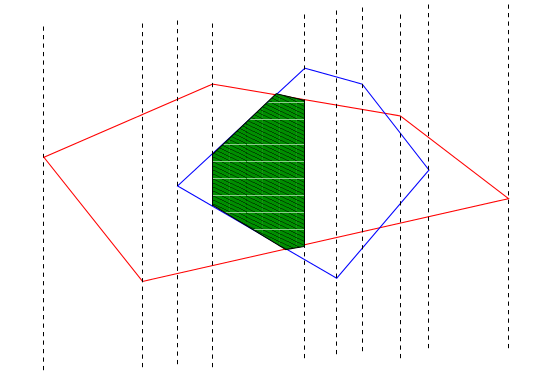
\includegraphics[scale=0.5]{img/ShamosHoey76}
  \caption{Podział na pasy a przecięcie
    wielokątów.\label{img:ShamosHoey76}}
\end{figure}

Następnie w czasie liniowym łączymy uzyskane kawałki i usuwamy
nadmiarowe wierzchołki powstałe przy podziale płaszczyzny. Początkowy
podział płaszczyzny również możemy przeprowadzić w czasie liniowym,
tak więc złożoność czasowa całego algorytmu wynosi $O(n + m)$.

\section{Algorytm O'Rourke-Chien-Olson-Naddor}
Kolejna metoda, zaproponowana przez O'Rourke i in.~\cite{Orourke98},
jest rozwinięciem algorytmu naiwnego.

Załóżmy, że $P$ i $Q$ przecinają się, oraz oznaczmy ich przecięcie $P
\cap Q$ jako $R$. Przyjmijmy również, że żadne dwie krawędzie z $P$ i
$Q$ nie są do siebie równoległe. Zauważmy, że brzeg $R$ składa się z
ciągu krawędzi należących do $P$, a następnie z ciągu krawędzie
należących do $Q$ (rysunek~\ref{img:sickles}). Jeżeli dany fragment
brzegu $R$ należy do $Q$, to jest on ,,objęty'' na zewnątrz przez ciąg
krawędzi $P$. I na odwrót --- fragmenty brzegu $R$, które należą do
$P$, są otoczone przez krawędzie należące do~$Q$.

\begin{figure}[htb]
  \centering
  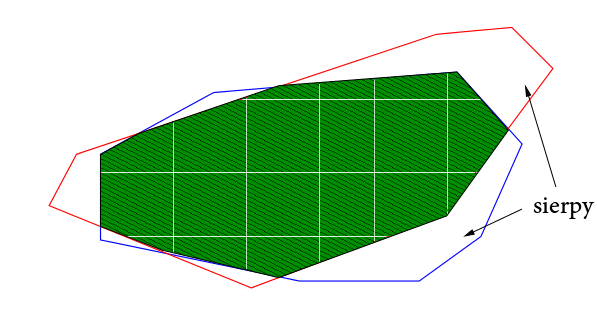
\includegraphics[scale=0.5]{img/Orourke98}
  \caption{Sierpy a przecięcie wielokątów.\label{img:sickles}}
\end{figure}

Możemy zauważyć, że przechodząc w odpowiedniej kolejności,
jednocześnie po zewnętrznych i wewnętrznych krawędziach ,,sierpa''
(rysunek~\ref{img:sickles}) ograniczymy sprawdzanie przecięć jedynie
do krawędzi początkowych i końcowych danego sierpa. Z tego względu
przy wyborze krawędzi, do której mamy przejść w danym kroku, kierujemy
się tym, czy krawędź bieżąca może zawierać przecięcie, które dopiero
ma być wykryte. Algorytm można przedstawić w postaci pseudokodu z
listingu~\ref{alg:Orourke98}.

\begin{figure}[htp]

  \begin{algorithmic}[1]
    \Procedure{Intersection of Convex Polygons}{}

    \State {$A \gets (p_0, p_1) \in P$}
    \State {$B \gets (q_0, q_1) \in Q$}

    \Repeat
    \State {sprawdź przecięcie krawędzi $A$ z krawędzią $B$}
    \State {w zależności od warunków przejdź po $A$ lub po $B$}
    \Until {$A$ i $B$ nie ,,okrążą'' swoich wielokątów}

    \EndProcedure
  \end{algorithmic}
  \caption{Algorytm wyznaczania przecięcia metodą O'Rourke i
    in.\label{alg:Orourke98}}
\end{figure}

Wybierzmy dowolną krawędź $A \in P$ oraz dowolną krawędź $B \in
Q$. Będziemy przechodzić po krawędziach obu wielokątów w kierunku
przeciwnym do ruch wskazówek zegara. W każdym kroku sprawdzamy
przecięcie bieżących krawędzi wielokątów $P$ i $Q$, i wybieramy
krawędź, do której podążymy w następnym kroku.  Chcemy kierować się
następującą regułą: jeżeli krawędź $B$ jest ,,skierowana'' w kierunku
krawędzi $A$, ale jej nie przecina, to zbliżamy się do $A$ przechodząc
po krawędzi $B$ w miejsce możliwego przecięcia, w przeciwnym przypadku
przechodzimy po $A$.

\begin{figure}[htb]
  \centering
  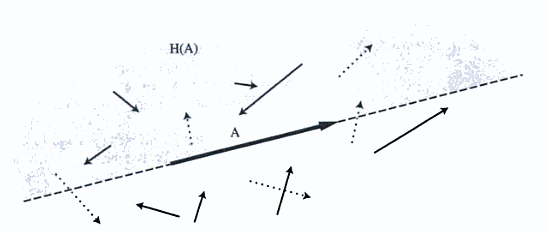
\includegraphics[scale=0.7]{img/vectors}
  \caption{\label{img:advance} Wektory krawędzi wielokątów $P$ i $Q$.}
\end{figure}

Rozważmy sytuację z rysunku~\ref{img:advance}. Niech $H(A)$ oznacza
półpłaszczyznę po lewej stronie skierowanej prostej współliniowej do
krawędzi $A$. Pogrubiona strzałka to wektor krawędzi $A$, pozostałe to
wektory krawędzi $B$.  Jako $A \times B > 0$ zapiszmy warunek taki, że
współrzędna $z$ iloczynu wektorowego wektorów krawędzi $A$ i $B$ jest
dodatnia (na rysunku~\ref{img:advance} oznaczone linią ciągłą). Jako
$a$ oznaczmy ,,skierowany'' wierzchołek należący do krawędzi $A$, zaś
jako $b$ ,,skierowany'' wierzchołek należący do krawędzi $B$. Przy
wyborze krawędzi, po której przejdziemy w bieżącym kroku, stosujemy
poniższą regułę. Jeżeli

\begin{center}
  $A \times B > 0 $ i $b \notin H(A)$ lub $A \times B < 0 $ i $b \in
  H(A)$,
\end{center}

to przechodzimy po $B$. W przypadku przeciwnym przechodzimy po $A$.

Jeżeli $P$ i $Q$ przecinają się, to przecięcie zostanie znalezione po
$O(n+m)$ krokach. Znając punkty przecięć, dodatkowe $n+m$ kroków
wystarcza do wyznaczenia wszystkich wierzchołków tworzących brzeg
przecięcia $P \cap Q$. Możemy tym samym stwierdzić, że jeżeli po
$2(n+m)$ krokach nie odnajdziemy przecięcia, to krawędzie $P$ i $Q$
nie przecinają się. Na koniec, jeżeli nie odnotowano przecięcia
krawędzi, pozostaje sprawdzanie trzech końcowych warunków z
listingu~\ref{alg:OrourkeFinalTerms}. Sprawdzenie, czy punkt zawiera
się w wielokącie, tak jak to zostało pokazane w
rozdziale~\ref{chap:point_location}, dla wielokąta prostego można
wykonać w czasie liniowym, stąd złożoność czasowa całego algorytmu
wynosi $O(n + m)$.

\begin{figure}
  \begin{algorithmic}[1]
    \If {$p_0$ leży w $Q$}
    \State $P$ zawiera się $Q$
    \Else
    \If {$q_0$ leży w $P$}
    \State $Q$ zawiera się $P$
    \Else
    \State $P$ i $Q$ nie przecinają się
    \EndIf
    \EndIf
  \end{algorithmic}
  \caption{\label{alg:OrourkeFinalTerms} Procedura sprawdzająca czy $P
    \subseteq Q$ lub $Q \subseteq P$, gdy nie wykryto przecięcia
    krawędzi.}
\end{figure}

\section{Algorytm Toussainta}
Stosunkowo prosty koncepcyjnie i implementacyjnie algorytm, działający
w czasie liniowym, zaproponował Toussaint w~\cite{ToussaintInt}.

\begin{figure}[htb]
  \centering
  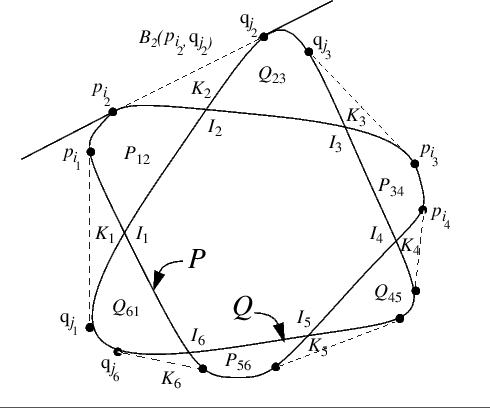
\includegraphics[scale=0.7]{img/toussaint1}
  \caption{\label{img:toussaint1} Kieszenie a przecięcie wielokątów.}
\end{figure}

\subsection{Opis}
Rozważmy dwa przecinające się wypukłe wielokąty $P$ i $Q$ oraz otoczkę
wypukłą sumy tych wielokątów $CH(P \cup Q)$
(rysunek~\ref{img:toussaint1}). Niech brzegi $P$ i $Q$ przecinają się
w $k$ punktach $I_1, I_2, \ldots, I_k$ ponumerowanych zgodnie z ruchem
wskazówek zegara. Brzegi $P$ i $Q$ oraz otoczka wypukła $CH(P \cup Q)$
dzielą płaszczyznę na $2k + 1$ ograniczonych regionów: obszar
przecięcia wielokątów $P \cap Q$ wyznaczony przez punkty $I_1, I_2,
\ldots, I_k$, następnie $k$ regionów gdzie $P$ lub $Q$ należy do
otoczki wypukłej $CH(P \cup Q)$, ale nie należy do obszaru $P \cap Q$
przecięcia tych wielokątów, oraz analogiczne $k$ ,,kieszeni'' $K_1,
K_2, \ldots, K_k$ leżących wewnątrz otoczki wypukłej $CH(P \cup Q$),
ale leżących na zewnątrz $P \cup Q$. Każdej kieszeni $K_v$
przypisujemy odpowiadający jej punkt przecięcia $I_v$ oraz krawędź
otoczki $CH(P \cup Q)$, którą będziemy nazywać \emph{mostem}, łączącą
wierzchołek $p_i$ wielokąta $P$ oraz wierzchołek $q_j$ wielokąta $Q$ i
oznaczymy ją jako $B_{v}(p_{i_v}, q_{j_v})$. Cały algorytm
wyznaczający przecięcie wielokątów $P$ i $Q$ można przedstawić w
trzech krokach (listing~\ref{alg:interconpol}).

\begin{figure}[htp]
  \begin{algorithmic}[1]
    \Procedure{Alogrytm Interconpol}{}

    \State \emph{/* krok 1 */}

    \State wyznacz otoczkę wypukłą $CH(P \cup Q)$

    \State

    \If {$CH(P \cup Q) = P$ (lub $Q$)}
    \State zwróć $Q$ (lub $P$) jako przecięcie

    \Else
    \State kontynuuj
    \EndIf

    \State

    \State \emph{/* krok 2 */}

    \State \textbf{dla każdego} mostu z $CH(P \cup Q)$:
    \State \hspace{\algorithmicindent} znajdź odpowiadający mu punkt
    przecięcia
    \State \textbf{end}

    \State

    \State \emph{/* krok 3 */}

    \State połącz wewnętrzne łańcuchy należące do $P$ i $Q$

    wyznaczone przez punkty przecięcia znalezione w poprzednim kroku

    \EndProcedure
  \end{algorithmic}
  \caption{\label{alg:interconpol} Algorytm wyznaczający przecięcie
    wielokątów metodą Toussainta.}
\end{figure}


\subsection{Poprawność}
Poprawność algorytmu opiera się na poniższych lematach.

\begin{lemat}\em{\cite{ToussaintInt}}
  Jeżeli $P$ i $Q$ przecinają się to dla każdego mostu $CH(P \cup Q)$
  istnieje jeden związany z nim punkt przecięcia $P \cap Q$.
\end{lemat}

\begin{proof}
  Oznaczmy jako $L(u, v)$ skierowaną prostą przechodzącą przez $u$ i
  $v$ w kierunku z $u$ do $v$, oraz oznaczmy jako $RH(u, v)$
  półpłaszczyznę na prawo od $L(u, v)$. Analogicznie, jako $LH(u, v)$
  oznaczmy półpłaszczyznę leżącą na lewo od $L(u, v)$.

  Niech $B(p_i, q_j)$ będzie mostem
  (rysunek~\ref{img:toussaint2}). $L(p_i, q_j)$ jest prostą
  wspierającą dla $P$ i $Q$ jednocześnie, więc $P$ i $Q$ muszą leżeć w
  półpłaszczyźnie $RH(p_i, q_j)$. Przejdźmy po brzegu $P$ zaczynając
  od $p_i$ w kierunku zgodnym z ruchem wskazówek zegara, dopóki nie
  natrafimy na krawędź wielokąta $P$ przecinającą krawędź wielokąta
  $Q$. Punkt przecięcia oznaczmy jako $I$. Analogicznie przejdźmy po
  brzegu $Q$ zaczynając od $q_j$ w kierunku przeciwnym do ruchu
  wskazówek zegara, dopóki nie natrafimy na krawędź wielokąta $Q$
  przecinającą krawędź wielokąta $P$. Z wypukłości obu wielokątów
  wynika, że tym razem punktem przecięcia również jest $I$ i w ten
  sposób jest on związany z mostem $B(p_i, q_j)$.

  Z drugiej strony załóżmy, że $I$ jest pewnym punktem przecięcia
  pomiędzy krawędziami $(p_k, p_{k+1}) \in P$ i $(q_l, q_{l+1}) \in
  Q$. Ponieważ $P \in RH(p_k, p_{k+1})$ oraz $Q \in RH(q_l, q_{l+1})$,
  to żadna krawędź inna niż $(p_k, p_{k+1})$ i $(q_l, q_{l+1})$ nie
  może przecinać się w regionie $R = RH(p_{k+1}, p_k) \cap RH(q_{l+1},
  q_l)$. Dodatkowo, ponieważ $\angle p_{k}Iq_{l+1} < 180^{\circ}$,
  musi istnieć krawędź $(p_i, q_j) \in CH(P \cup Q)$, która przecina
  region $R$ i jest nią most odpowiadający punktowi przecięcia $I$.
\end{proof}

\begin{figure}[htb]
  \centering
  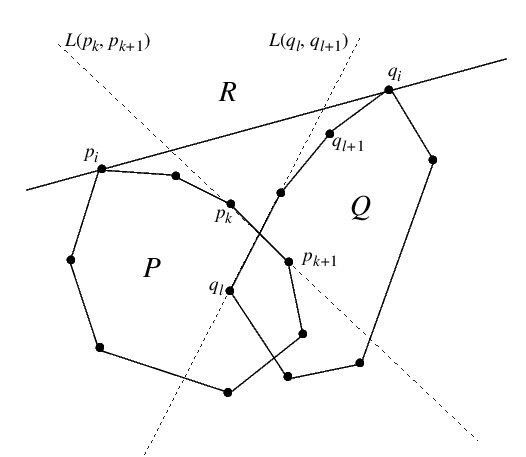
\includegraphics[scale=0.7]{img/toussaint2}
  \caption{\label{img:toussaint2} Most a punkt przecięcia.}
\end{figure}

\begin{twierdzenie}[Toussaint 1985\label{thm:toussaint85}]
  Opisany wyżej algorytm poprawnie wyznacza punkt przecięcia dla
  odpowiadającego mu mostu.
\end{twierdzenie}

Zanim omówimy dowód powyższego twierdzenia wprowadźmy kilka definicji.

\begin{definicja}
  \emph{Łańcuchem} $C(p_i,p_{i+1},\ldots,p_j)$ nazywamy ciąg
  kolejnych, następujących po sobie krawędzi i wierzchołków wielokąta
  prostego zaczynając od wierzchołka $p_i$ do wierzchołka
  $p_j$. Jeżeli każda krawędź łańcucha wraz z następną krawędzią
  tworzy kąt prawoskrętny, to taki łańcuch nazywamy
  \emph{wypukłym}. Analogicznie, jeżeli każda krawędź wraz ze swoim
  następnikiem tworzy kąt lewoskrętny, to taki łańcuch nazywamy
  \emph{łańcuchem wklęsłym}.
\end{definicja}

\begin{definicja}
  Wielokątem \emph{żaglokształtnym} nazywamy wielokąt zawierający
  krawędź $(p_{i}p_{i+1})$ będącą \emph{masztem} oraz wierzchołek
  $p_j$ (tzw.\ \emph{czubek żagla}) połączony z wierzchołkami $p_i$ i
  $p_{i+1}$ łańcuchami wklęsłymi.
\end{definicja}

\begin{definicja}
  Odcinek leżący w wielokącie $P$ i łączący dwa nie sąsiadujące
  wierzchołki wielokąta $P$ nazywamy \emph{przekątną} $P$.
\end{definicja}

\begin{definicja}\label{def:ear}
  Niech $p_i, p_{i+1}, p_{i+2}$ będą trzema kolejnymi, następującymi
  po sobie wierzchołkami należącymi do wielokąta $P$. Jeżeli przekątna
  łącząca $p_{i}$ i $p_{i+2}$ leży w $P$, to punkt $p_i$ nazywamy
  \emph{uchem} wielokąta $P$.
\end{definicja}

Zauważmy, że każda kieszeń wraz z odpowiadającym jej mostem oraz
punktem przecięcia $I_i$ tworzy wielokąt
\emph{żaglokształtny}. Ponadto mamy następujący lemat.

\begin{lemat}\label{lem:sailtip}\emph{\cite{ToussaintInt}}
  Czubek wielokąta żaglokształtnego jest uchem.
\end{lemat}

\begin{figure}[htb]
  \centering
  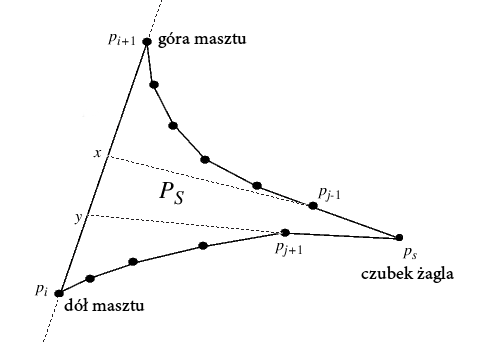
\includegraphics[scale=0.7]{img/toussaint3}
  \caption{\label{img:toussaint3} Wielokąt żaglokształtny.}
\end{figure}

\begin{proof}
  Przedłużmy krawędzie $(p_j,p_{j-1})$ i $(p_j, p_{j+1})$ tak, by
  przecinały prostą $L(p_i, p_{i+1})$ odpowiednio w punktach $x$ i $y$
  (rysunek~\ref{img:toussaint3}). Ze względu na to, że $p_j$ jest
  połączony z $p_i$ łańcuchem wypukłym, punkt $x$ musi leżeć na
  odcinku $(p_i, p_{i+1})$ będącym masztem $P$. Analogicznie, punkt
  $y$ musi leżeć na maszcie $P$. Punkty $p_j, p_{j-1}, x, y, p_{j+1},
  p_j$, tworzą obszar znajdujący się w całości w $P$, stąd przekątna
  $(p_{j-1}, p_{j+1})$ również musi leżeć w $P$.
\end{proof}

\begin{twierdzenie}[Meisters 1975\label{thm:meisters}] Każdy wielokąt o
  $n$ krawędziach ($n > 3$) ma co najmniej dwoje nienachodzących na
  siebie uszu.
\end{twierdzenie}

\begin{lemat}\label{lem:sailmast}\emph{\cite{ToussaintInt}}
  Uchem jest góra masztu wielokąta żaglokształtnego albo uchem jest
  jego dół.
\end{lemat}

\begin{proof}
  Z definicji~\ref{def:ear} wiemy, że tylko wierzchołki wypukłe mogą
  być uszami, a więc w wielokącie żaglokształtnym $P$ uszami mogą być
  jedynie $p_i$, $p_{i+1}$ oraz $p_j$. Z lematu~\ref{lem:sailtip}
  wiemy, że $p_j$ musi być uchem. Z twierdzenia~\ref{thm:meisters}
  wiemy, że $P$ musi mieć co najmniej dwoje uszu. Stąd albo $p_i$ albo
  $p_{i+1}$ musi być uchem.
\end{proof}

\begin{proof}[Dowód twierdzenia~\ref{thm:toussaint85}]
  W każdym kroku algorytmu znajdującego przecięcie krawędzi wielokąta
  $P$ i wielokąta $Q$ zachowywany jest następujący niezmiennik: po
  obcięciu kolejnego ucha wielokąta żaglokształtnego pozostała cześć
  wielokąta również jest wielokątem żaglokształtnym.

  Lemat~\ref{lem:sailtip} pozwala nam na triangulację $P$ w każdym
  kroku obcinając ucho będące górą lub dołem masztu, dopóki nie
  dojdziemy do czubka żagla i krawędzi z niego wychodzących.
\end{proof}

W naszym przypadku wierzchołek $p_j$ jest szukanym punktem przecięcia
$I_i$, tak więc dodatkowo w algorytmie powinniśmy uwzględnić warunek
sprawdzający, czy w bierzącym kroku nadal rozważamy krawędź należącą
do wielokąta żaglokształtnego. Kompletny algorytm znajdujący czubek
żagla wielokąta $P$ został przedstawiony na
listingu~\ref{alg:stepdown}.

\begin{figure}[htp]
  \begin{algorithmic}[1]
    \Procedure{Stepdown}{}

    \State $i \gets 1$
    \State $j \gets 1$

    % \State

    \Repeat
    \State $koniec \gets true$

    % \State

    \While{$\angle p_{i}p_{i+1}q_{j+1}$ jest lewoskrętny}
    \State $j \gets j + 1$
    \State $koniec \gets false$
    \EndWhile

    % \State

    \While{$\angle q_{j}q_{j+1}p_{i+1}$ jest prawoskrętny}
    \State $i \gets i + 1$
    \State $koniec \gets false$
    \EndWhile

    \Until{$koniec$}

    % \State

    \State $p_s \gets p_i$
    \State $q_t \gets q_j$

    \EndProcedure
  \end{algorithmic}
  \caption{\label{alg:stepdown} Algorytm znajdujący punkt przecięcia
    krawędzi wielokątów $P$ i $Q$ związany z danym mostem.}
\end{figure}

Wejściem dla procedury jest most $B_k(p_i,p_j)$ należący do $CH(P \cup
Q)$, a wyjściem para wierzchołków $p_s$ i $q_t$, gdzie $(p_s,p_{s+1})
\cap (q_t,q_{t+1})$ wyznacza punkt przecięcia $I_k$. Warunki ,,$\angle
p_{i}p_{i+1}q_{j+1}$ jest lewoskrętny'' oraz ,,$\angle
q_{j}q_{j+1}p_{i+1}$ jest prawoskrętny'' w pętlach \textbf{while}
zapewniają, że w każdym kroku odetniemy ucho oraz że nie przejdziemy
przez czubek żagla. Przebieg działania procedury \textsc{Stepdown} dla
mostu z rysunku~\ref{fig:bridge} przedstawiają
rysunki~\ref{fig:stepdown1}--\ref{fig:stepdown5}.

\subsection{Złożoność}
Niech $n$ oznaczana liczbę wierzchołków wielokąta $P$, a $m$ liczbę
wierzchołków wielokąta $Q$. Znalezienie otoczki wypukłej dwóch
przecinających się wielokątów wypukłych może być wykonane w czasie
$O(m + n)$~\cite{Toussaint83}. W~\cite{ToussaintInt} Toussaint
proponuje wykorzystać technikę \emph{rotating calipers}, pozwalającą w
tym samym czasie stwierdzić, czy $CH(P \cup Q) = P$ lub $CH(P \cup Q)
= Q$.

Procedura znajdująca przecięcie $I_k$ jest wywoływana $k$ razy. Każde
wywołanie wymaga czasu liniowego zależnego od liczby wierzchołków
należących do danego żagla. Wszystkich takich wierzchołków może być
maksymalnie $n + m$, stąd ta część algorytmu wymaga czasu $O(n + m)$.

Ostatnią część algorytmu, tj.\ połączenie uzyskanych łańcuchów
wewnętrznych można wykonać w czasie liniowym przechodząc przez
krawędzie obydwu wielokątów, jeżeli podczas szukania punktów przecięć
oznaczyliśmy kierunek, w którym dana część wielokąta staje się
łańcuchem wewnętrznym.

Stąd złożoność czasowa całego algorytmu wynosi $O(n + m)$.

\begin{figure}[tp]
  \centering
  \begin{tikzpicture}
    \coordinate (q4) at (6, 5);
    \coordinate (q3) at (4, 4.5);
    \coordinate (q2) at (2.5, 3.5);
    \coordinate (q1) at (1.5, 1.5);
    \coordinate (q0) at (2, -0.25);
    \coordinate (q6) at (5, 0);
    \coordinate (q5) at (7, 2);

    \draw [blue] (q0) -- (q1) -- (q2) -- (q3) -- (q4) --  (q5) -- (q6) -- cycle;

    \node [anchor=center,circle,draw,fill,inner sep=1pt,
    label={250:$q_0$}] at (q0) {};

    \node [anchor=center,circle,draw,fill,inner sep=1pt,
    label={left:$q_1$}] at (q1) {};

    \node [anchor=center,circle,draw,fill,inner
    sep=1pt,label={right:$q_2$}] at (q2) {};

    \node [anchor=center,circle,draw,fill,inner
    sep=1pt,label={below:$q_3$}] at (q3) {};

    \node [anchor=center,circle,draw,fill,inner
    sep=1pt,label={above:$q_4$}] at (q4) {};

    \node [anchor=center,circle,draw,fill,inner
    sep=1pt,label={right:$q_5$}] at (q5) {};

    \node [anchor=center,circle,draw,fill,inner
    sep=1pt,label={below:$q_6$}] at (q6) {};

    \coordinate (p4) at (2, 3);
    \coordinate (p3) at (1, 4.5);
    \coordinate (p2) at (-1, 5);
    \coordinate (p1) at (-3, 3);
    \coordinate (p0) at (0, 0);
    \coordinate (p5) at (2, 1);

    \draw [red] (p0) -- (p1) -- (p2) -- (p3) --  (p4) -- (p5) -- cycle;

    \node [anchor=center,circle,draw,fill,inner sep=1pt,
    label={right:$p_1$}] at (p1) {};

    \node [anchor=center,circle,draw,fill,inner
    sep=1pt,label={above:$p_2$}] at (p2) {};

    \node [anchor=center,circle,draw,fill,inner
    sep=1pt,label={below:$p_3$}] at (p3) {};

    \node [anchor=center,circle,draw,fill,inner
    sep=1pt,label={left:$p_4$}] at (p4) {};

    \node [anchor=center,circle,draw,fill,inner
    sep=1pt,label={right:$p_5$}] at (p5) {};

    \node [anchor=center,circle,draw,fill,inner
    sep=1pt,label={below:$p_0$}] at (p0) {};

    \draw [dashed, shorten >= -2cm, shorten <= -2cm] (p2) -- (q4);
  \end{tikzpicture}
  \caption{Przerywaną linią oznaczono most.\label{fig:bridge}}
\end{figure}


\begin{figure}[htp]
  \centering
  \begin{tikzpicture}
    \coordinate (q4) at (6, 5);
    \coordinate (q3) at (4, 4.5);
    \coordinate (q2) at (2.5, 3.5);
    \coordinate (q1) at (1.5, 1.5);
    \coordinate (q0) at (2, -0.25);
    \coordinate (q6) at (5, 0);
    \coordinate (q5) at (7, 2);

    \draw [blue] (q1) -- (q2) -- (q3) -- (q4);

    \node [anchor=center,circle,draw,fill,inner sep=1pt,
    label={}] at (q1) {};

    \node [anchor=center,circle,draw,fill,inner
    sep=1pt,label={}] at (q2) {};

    \node [anchor=center,circle,draw,fill,inner
    sep=1pt,label={below:$q_{j+1}$}] at (q3) {};

    \node [anchor=center,circle,draw,fill,inner
    sep=1pt,label={above:$q_j$}] at (q4) {};

    \coordinate (p4) at (2, 3);
    \coordinate (p3) at (1, 4.5);
    \coordinate (p2) at (-1, 5);
    \coordinate (p1) at (-3, 3);
    \coordinate (p0) at (0, 0);
    \coordinate (p5) at (2, 1);

    \draw [red] (p2) -- (p3) --  (p4) -- (p5);

    \node [anchor=center,circle,draw,fill,inner
    sep=1pt,label={above:$p_i$}] at (p2) {};

    \node [anchor=center,circle,draw,fill,inner
    sep=1pt,label={left:$p_{i+1}$}] at (p3) {};

    \node [anchor=center,circle,draw,fill,inner
    sep=1pt,label={}] at (p4) {};

    \node [anchor=center,circle,draw,fill,inner
    sep=1pt,label={}] at (p5) {};

    \draw (p2) -- (q4);
    \draw [dashed] (p2) -- (q3);
  \end{tikzpicture}
  \caption{Kąt $\angle{p_{i}p_{i+1}q_{j+1}}$ jest lewoskrętny, więc
    odcinamy ucho $q_j$.\label{fig:stepdown1}}
\end{figure}

\begin{figure}[htp]
  \centering
  \begin{tikzpicture}
    \coordinate (q4) at (6, 5);
    \coordinate (q3) at (4, 4.5);
    \coordinate (q2) at (2.5, 3.5);
    \coordinate (q1) at (1.5, 1.5);
    \coordinate (q0) at (2, -0.25);
    \coordinate (q6) at (5, 0);
    \coordinate (q5) at (7, 2);

    \draw [blue] (q1) -- (q2) -- (q3) -- (q4);

    \node [anchor=center,circle,draw,fill,inner sep=1pt,
    label={}] at (q1) {};

    \node [anchor=center,circle,draw,fill,inner
    sep=1pt,label={}] at (q2) {};

    \node [anchor=center,circle,draw,fill,inner
    sep=1pt,label={below:$q_{j}$}] at (q3) {};

    \node [anchor=center,circle,draw,fill,inner
    sep=1pt,label={right:$q_{j+1}$}] at (q2) {};

    \coordinate (p4) at (2, 3);
    \coordinate (p3) at (1, 4.5);
    \coordinate (p2) at (-1, 5);
    \coordinate (p1) at (-3, 3);
    \coordinate (p0) at (0, 0);
    \coordinate (p5) at (2, 1);

    \draw [red] (p2) -- (p3) --  (p4) -- (p5);

    \node [anchor=center,circle,draw,fill,inner
    sep=1pt,label={above:$p_i$}] at (p2) {};

    \node [anchor=center,circle,draw,fill,inner
    sep=1pt,label={left:$p_{i+1}$}] at (p3) {};

    \node [anchor=center,circle,draw,fill,inner
    sep=1pt,label={}] at (p4) {};

    \node [anchor=center,circle,draw,fill,inner
    sep=1pt,label={}] at (p5) {};

    \draw (p2) -- (q3);
    \draw [dashed] (q3) -- (p3);
  \end{tikzpicture}
  \caption{Kąt $\angle{q_{j}q_{j+1},p_{i+1}}$ jest prawoskrętny, więc
    odcinamy ucho $p_i$.}
\end{figure}

\begin{figure}[htp]
  \centering
  \begin{tikzpicture}
    \coordinate (q4) at (6, 5);
    \coordinate (q3) at (4, 4.5);
    \coordinate (q2) at (2.5, 3.5);
    \coordinate (q1) at (1.5, 1.5);
    \coordinate (q0) at (2, -0.25);
    \coordinate (q6) at (5, 0);
    \coordinate (q5) at (7, 2);

    \draw [blue] (q1) -- (q2) -- (q3) -- (q4);

    \node [anchor=center,circle,draw,fill,inner sep=1pt,
    label={}] at (q1) {};

    \node [anchor=center,circle,draw,fill,inner
    sep=1pt,label={}] at (q2) {};

    \node [anchor=center,circle,draw,fill,inner
    sep=1pt,label={below:$q_{j}$}] at (q3) {};

    \node [anchor=center,circle,draw,fill,inner
    sep=1pt,label={right:$q_{j+1}$}] at (q2) {};

    \coordinate (p4) at (2, 3);
    \coordinate (p3) at (1, 4.5);
    \coordinate (p2) at (-1, 5);
    \coordinate (p1) at (-3, 3);
    \coordinate (p0) at (0, 0);
    \coordinate (p5) at (2, 1);

    \draw [red] (p2) -- (p3) --  (p4) -- (p5);

    \node [anchor=center,circle,draw,fill,inner
    sep=1pt,label={}] at (p2) {};

    \node [anchor=center,circle,draw,fill,inner
    sep=1pt,label={left:$p_{i}$}] at (p3) {};

    \node [anchor=center,circle,draw,fill,inner
    sep=1pt,label={left:$p_{i+1}$}] at (p4) {};

    \node [anchor=center,circle,draw,fill,inner
    sep=1pt,label={}] at (p5) {};

    \draw (q3) -- (p3);
    \draw [dashed] (p3) -- (q2);

  \end{tikzpicture}
  \caption{Kąt $\angle{p_{i}p_{i+1}q_{j+1}}$ jest lewoskrętny, więc
    odcinamy ucho $q_j$.}
\end{figure}

\begin{figure}[htp]
  \centering
  \begin{tikzpicture}
    \coordinate (q4) at (6, 5);
    \coordinate (q3) at (4, 4.5);
    \coordinate (q2) at (2.5, 3.5);
    \coordinate (q1) at (1.5, 1.5);
    \coordinate (q0) at (2, -0.25);
    \coordinate (q6) at (5, 0);
    \coordinate (q5) at (7, 2);

    \draw [blue] (q1) -- (q2) -- (q3) -- (q4);

    \node [anchor=center,circle,draw,fill,inner sep=1pt,
    label={250:$q_{j+1}$}] at (q1) {};

    \node [anchor=center,circle,draw,fill,inner
    sep=1pt,label={}] at (q3) {};

    \node [anchor=center,circle,draw,fill,inner
    sep=1pt,label={right:$q_{j}$}] at (q2) {};

    \coordinate (p4) at (2, 3);
    \coordinate (p3) at (1, 4.5);
    \coordinate (p2) at (-1, 5);
    \coordinate (p1) at (-3, 3);
    \coordinate (p0) at (0, 0);
    \coordinate (p5) at (2, 1);

    \draw [red] (p2) -- (p3) --  (p4) -- (p5);

    \node [anchor=center,circle,draw,fill,inner
    sep=1pt,label={}] at (p2) {};

    \node [anchor=center,circle,draw,fill,inner
    sep=1pt,label={left:$p_{i}$}] at (p3) {};

    \node [anchor=center,circle,draw,fill,inner
    sep=1pt,label={left:$p_{i+1}$}] at (p4) {};

    \node [anchor=center,circle,draw,fill,inner
    sep=1pt,label={}] at (p5) {};

    \draw (p3) -- (q2);
    \draw [dashed] (p4) -- (q2);
  \end{tikzpicture}
  \caption{Kąt $\angle{q_{j}q_{j+1}p_{i+1}}$ jest prawoskrętny, więc
    odcinamy ucho $p_i$.}
\end{figure}

\begin{figure}[htp]
  \centering
  \begin{tikzpicture}
    \coordinate (q4) at (6, 5);
    \coordinate (q3) at (4, 4.5);
    \coordinate (q2) at (2.5, 3.5);
    \coordinate (q1) at (1.5, 1.5);
    \coordinate (q0) at (2, -0.25);
    \coordinate (q6) at (5, 0);
    \coordinate (q5) at (7, 2);

    \draw [blue] (q1) -- (q2) -- (q3) -- (q4);

    \node [anchor=center,circle,draw,fill,inner sep=1pt,
    label={250:$q_{j+1}$}] at (q1) {};

    \node [anchor=center,circle,draw,fill,inner
    sep=1pt,label={}] at (q3) {};

    \node [anchor=center,circle,draw,fill,inner
    sep=1pt,label={right:$q_{j}$}] at (q2) {};

    \coordinate (p4) at (2, 3);
    \coordinate (p3) at (1, 4.5);
    \coordinate (p2) at (-1, 5);
    \coordinate (p1) at (-3, 3);
    \coordinate (p0) at (0, 0);
    \coordinate (p5) at (2, 1);

    \draw [red] (p2) -- (p3) --  (p4) -- (p5);

    \node [anchor=center,circle,draw,fill,inner
    sep=1pt,label={}] at (p2) {};

    \node [anchor=center,circle,draw,fill,inner
    sep=1pt,label={}] at (p3) {};

    \node [anchor=center,circle,draw,fill,inner
    sep=1pt,label={left:$p_{i}$}] at (p4) {};

    \node [anchor=center,circle,draw,fill,inner
    sep=1pt,label={right:$p_{i+1}$}] at (p5) {};

    \draw (p4) -- (q2);
  \end{tikzpicture}
  \caption{Kąt $\angle{p_{i}p_{i+1}q_{j+1}}$ jest prawoskrętny, a kąt
    $\angle{q_{j}q_{j+1}p_{i+1}}$ lewoskrętny, zatem algorytm kończy
    działanie.\label{fig:stepdown5}}
\end{figure}

%%% Local Variables:
%%% mode: latex
%%% TeX-master: "masterthesis"
%%% TeX-engine: xetex
%%% End:
